\subsection{Matrices del sistema}
La matriz $\Lambda$ de coeficientes de desintegración del sistema es un arreglo disperso. A continuación se muestra dejando en blanco aquellos elementos valuados en 0:

\begin{equation}
	\Lambda=\left(\begin{smallmatrix}
		-\lambda_1& & & & & & & & & & & & & & \\
		 \lambda_1&-\lambda_2& & & & & & & & & & & & & \\
		 & \lambda_2&-\lambda_3& & & & & & & & & & & & \\
		 & & \lambda_3&-\lambda_4& & & & & & & & & & & \\
		 & & &\lambda_{4,\beta}&-\lambda_5& & & & & & & & & & \\
		 & & &\lambda_{4, \alpha}& &-\lambda_6& & & & & & & & & \\
		 & & & & \lambda_5& \lambda_6&-\lambda_7& & & & & & & & \\
		 & & & & & & \lambda_7&-\lambda_8& & & & & & & \\
		 & & & & & & & \lambda_8&-\lambda_9& & & & & & \\
		 & & & & & & & &\lambda_{9,\alpha}&-\lambda_{10}& & & & & \\
		 & & & & & & & &\lambda_{9, \beta}& &-\lambda_{11}& & & & \\
		 & & & & & & & & & \lambda_{10}&\lambda_{11}&-\lambda_{12}& & & \\
		 & & & & & & & & & & &\lambda_{12, \beta}&-\lambda_{13}& & \\
		 & & & & & & & & & & &\lambda_{12, \alpha}& &-\lambda_{14}& \\ 
		 & & & & & & & & & & & &\lambda_{13}&\lambda_{14}& 0\\
	\end{smallmatrix}\right)
\end{equation}\label{matriz_determinista}

Para la versión estocástica del sistema, se toma como término determinista la matriz $\mathcal{L}$ y las matrices estocásticas $\mathcal{X}$, $\mathcal{Y}$ y $\mathcal{Z}$ dadas por los siguientes arreglos dispersos:

\begin{equation}
	\mathcal{L}=\left(\begin{smallmatrix}
		-\lambda_1& & & & & & & & & & & \\								%fila 1
		\lambda_1&-\lambda_2& & & & & & & & & & \\						%fila 2
		&\lambda_2&-\lambda_3& & & & & & & & & \\						%fila 3
		& & \lambda_3&-\lambda_4& & & & & & & & \\						%fila 4
		& & &\lambda_{4, \alpha}&-\lambda_6& & & & & & & \\				%fila 5
		& & & &\lambda_6 &-\lambda_7& & & & & & \\						%fila 6
		& & & & &\lambda_7&-\lambda_8& & & & & \\						%fila 7
		& & & & & &\lambda_8&-\lambda_9& & & & \\						%fila 8
		& & & & & & &\lambda_{9, \beta}&-\lambda_{11}& & & \\			%fila 9
		& & & & & & & &\lambda{11}&-\lambda_{12}& & \\					%fila 10
		& & & & & & & & &\lambda_{12, \beta}&-\lambda_{14}&\\			%fila 11 
		& & & & & & & & & &\lambda{14}& 0\\								%fila 12
	\end{smallmatrix}\right)\label{matriz_determinista_alternativa}
\end{equation}

\begin{equation}
	\mathcal{X}=\begin{cases}
		(\lambda_4-2\lambda_{4, \alpha}) & \textrm{En la fila 5, columna 4.}\\
		-\lambda_5+\lambda_6 & \textrm{En la fila 5, columna 5.}\\
		\lambda_5-\lambda_6 & \textrm{En la fila 6, columna 5.}
	\end{cases}\label{matriz_estocastica_x}
\end{equation}

\begin{equation}
	\mathcal{Y}=\begin{cases}
		-(\lambda_9-2\lambda_{9, \alpha}) & \textrm{En la fila 9, columna 8.}\\
		-\lambda_{10}+\lambda_{11} & \textrm{En la fila 9, columna 9.} \\
		\lambda_{10}-\lambda_{11} & \textrm{En la fila 10, columna 9.} \\
	\end{cases}\label{matriz_estocastica_y}
\end{equation}

\begin{equation}
	\mathcal{Z}=\begin{cases}
		(\lambda_{12}-2\lambda_{12, \alpha}) & \textrm{En la fila 11, columna 10.}\\
		-\lambda_{13}+\lambda_{14} & \textrm{En la fila 11, columna 11.}\\
		\lambda_{13}-\lambda_{14}  & \textrm{En la fila 12, columna 11.}\\
	\end{cases}\label{matriz_estocastica_z}
\end{equation}

\noindent donde se suponen 0 todos los elementos no especificados.
\newpage
\subsection{Tablas de coeficientes}
Los cuadros a continuación presentan las constantes de decaimiento de los radionúclidos de la serie del actínido, los coeficientes de linealización de la combinación lineal de los eigenvectores del sistema, y los coeficientes de Bateman de la serie, en ese orden. 

\begin{center}
	\noindent\begin{tabular}{|c|l|l|}
		\hline
		Radionúclido & \multicolumn{1}{c|}{$\tau_{1/2}$} & \multicolumn{1}{c|}{$\lambda\ (a^{-1})$} \\\hline\hline 
		$^{235}U$  & $\unit[7.04\times 10^8]{a}$ & $9.846\times 10^{-10}$ \\
		$^{231}Th$ & $\unit[25.52]{h}$ & $1.786\times 10^{-3}$ \\
		$^{231}Pa$ & $\unit[3.276\times 10^4]{a}$ & $2.116\times 10^{-5}$ \\
		$^{227}Ac$ & $\unit[21.772]{a}$ & $3.184\times 10^{-2}$ \\
		$^{227}Th$ & $\unit[18.697]{d}$ & $1.353\times 10^{1}$ \\
		$^{223}Fr$ & $\unit[22.00]{min}$ & $1.656\times 10^{4}$ \\
		$^{223}Ra$ & $\unit[11.43]{d}$ & $2.213\times 10^{1}$ \\
		$^{219}Rn$ & $\unit[3.96]{s}$ & $5.520\times 10^{6}$ \\
		$^{215}Po$ & $\unit[1.781\times 10^{-3}]{s}$ & $1.227\times 10^{10}$ \\
		$^{211}Pb$ & $\unit[36.1]{min}$ & $1.009\times 10^{4}$ \\
		$^{215}At$ & $\unit[0.10\times 10^{-3}]{s}$ & $2.186\times 10^{11}$ \\
		$^{211}Bi$ & $\unit[2.14]{min}$ & $1.702\times 10^{5}$ \\
		$^{211}Po$ & $\unit[0.516]{s}$ & $4.236\times 10^{7}$ \\
		$^{207}Tl$ & $\unit[4.77]{min}$ & $7.638\times 10^{4}$ \\
		$^{207}Pb$ & $\infty$ & $0.0000$\\\hline
	\end{tabular}
	\captionof{table}{Períodos de semidesintegración y constantes de decaimiento para cada radionúclido en la cadena del uranio-235. Datos según \textit{NuDat}.}
	\label{tabladeconstantesdedesintegracion}
\end{center}

\begin{center}
	\begin{tabular}{|c|l|}
		\hline
		$\kappa$-ésimo coeficiente & \multicolumn{1}{c|}{valor aproximado}\\\hline\hline
		$\kappa_1$ & $\ 1.0000$ \\
		$\kappa_2$ & $-1.7112\times 10^{-32}$ \\
		$\kappa_3$ & $\ 6.7401\times 10^{-34}$ \\
		$\kappa_4$ & $-1.5322\times 10^{-30}$ \\
		$\kappa_5$ & $-3.1814\times 10^{-29}$ \\
		$\kappa_6$ & $\ 4.3028\times 10^{-42}$ \\
		$\kappa_7$ & $-4.0795\times 10^{-35}$ \\
		$\kappa_8$ & $\ 2.6946\times 10^{-32}$ \\
		$\kappa_9$ & $\ 6.7765\times 10^{-24}$ \\
		$\kappa_{10}$ & $\ 1.5548\times 10^{-24}$ \\
		$\kappa_{11}$ & $\ 1.3446\times 10^{-29}$ \\
		$\kappa_{12}$ & $-1.7296\times 10^{-12}$ \\
		$\kappa_{13}$ & $-6.6619\times 10^{-5}$\\
		$\kappa_{14}$ & $-7.8436\times 10^{-7}$ \\
		$\kappa_{15}$ & $\ 1.4142$\\
		\hline
	\end{tabular}
	\captionof{table}{Constantes de integración del sistema \ref{sistemadinamicoU235} bajo la condición de frontera, ecuaciones \ref{condicioninicialpadre} y \ref{condicioninicialproductos}.}\label{tabladecoeficientes2}
\end{center}
\newpage
\begin{center}
\begin{tabular}[h]{|c|r|r|r|r|r|}
    \hline
    $N_i$ & $C_1^*$ & $C_2^*$ & $C_3^*$ & $C_4^*$ & $C_5^*$ \\\hline\hline
    $N_1$ & $1.0000$ & $0$ & $0$ & $0$ & $0$\\
    $N_2$ & $5.5129\times 10^{-7}$& $-5.5129\times 10^{-7}$ & $0$ & $0$ & $0$\\
    $N_3$ & $4.6533\times 10^{-5}$& $5.5790\times 10^{-7}$ & $-4.7091\times 10^{-5}$ & $0$ & $0$\\
    $N_4$ & $3.0925\times 10^{-8}$& $3.9280\times 10^{-10}$ & $-3.1316\times 10^{-8}$ & $-1.2221\times 10^{-12}$ & $0$\\
    $N_5$ & $1.0043\times 10^{-12}$& $1.2758\times 10^{-14}$ & $-1.0170\times 10^{-12}$ & $-3.9781\times 10^{-17}$ & $0$\\
    $N_6$ & $5.8639\times 10^{-14}$& $7.4481\times 10^{-16}$ & $-5.9381\times 10^{-14}$ & $-2.3173\times 10^{-18}$ & $9.5014\times 10^{-30}$\\
    $N_7$ & $4.4494\times 10^{-11}$& $5.6519\times 10^{-13}$ & $-4.5057\times 10^{-11}$ & $-1.7609\times 10^{-15}$ & $-9.5141\times 10^{-30}$\\
    $N_8$ & $1.7838\times 10^{-16}$& $2.2659\times 10^{-18}$ & $-1.8064\times 10^{-16}$ & $-7.0595\times 10^{-21}$ & $-3.8257\times 10^{-35}$\\
    $N_9$ & $8.0248\times 10^{-20}$& $1.0194\times 10^{-21}$ & $-8.1264\times 10^{-20}$ & $-3.1759\times 10^{-24}$ & $-1.7211\times 10^{-38}$\\
    $N_{10}$ & $9.7586\times 10^{-14}$& $1.2396\times 10^{-15}$ & $-9.8822\times 10^{-14}$ & $-3.8621\times 10^{-18}$ & $3.2640\times 10^{-32}$ \\
    $N_{11}$ & $1.0360\times 10^{-26}$& $1.3160\times 10^{-28}$ & $-1.0491\times 10^{-26}$ & $-4.1000\times 10^{-31}$ & $-2.2219\times 10^{-45}$\\
    $N_{12}$ & $5.7852\times 10^{-15}$& $7.3488\times 10^{-17}$ & $-5.8585\times 10^{-15}$ & $-2.2896\times 10^{-19}$ & $2.1436\times 10^{-33}$\\
    $N_{13}$ & $2.3181\times 10^{-17}$& $2.9446\times 10^{-19}$ & $-2.3474\times 10^{-17}$ & $-9.1739\times 10^{-22}$ & $8.5923\times 10^{-36}$\\
    $N_{14}$ & $3.5580\times 10^{-17}$& $4.5197\times 10^{-19}$ & $-3.6031\times 10^{-17}$ & $-1.4081\times 10^{-21}$ & $1.6833\times 10^{-35}$\\
    $N_{15}$ & $-1.0000$& $-7.0032\times 10^{-9}$ & $4.7123\times 10^{-5}$ & $1.2239\times 10^{-12}$ & $-2.2056\times 10^{-32}$\\
    \hline
\end{tabular}
\captionof{table}{Coeficientes de Bateman obtenidos mediante eigenvectores parte 1.}\label{tabla_coeficientes_bateman1}
\end{center}

\begin{center}
\begin{tabular}[h]{|c|r|r|r|r|r|}
    \hline
   $N_i$ & $C_6^*$ & $C_7^*$ & $C_8^*$ & $C_9^*$ & $C_{10}^*$  \\\hline\hline
   $N_1$ & $0$& $0$ & $0$ & $0$ & $0$\\
   $N_2$ & $0$& $0$ & $0$ & $0$ & $0$\\
   $N_3$ & $0$& $0$ & $0$ & $0$ & $0$\\
   $N_4$ & $0$& $0$ & $0$ & $0$ & $0$\\
   $N_5$ & $4.8886\times 10^{-25}$& $0$ & $0$ & $0$ & $0$\\
   $N_6$ & $0$ & $0$ & $0$ & $0$ & $0$\\
   $N_7$ & $7.6910\times 10^{-25}$ & $4.7861\times 10^{-24}$ & $0$ & $0$ & $0$\\
   $N_8$ & $3.0834\times 10^{-30}$ & $1.9188\times 10^{-29}$ & $1.9032\times 10^{-32}$ & $0$ & $0$\\
   $N_9$ & $1.3871\times 10^{-33}$ & $8.6322\times 10^{-33}$ & $8.5660\times 10^{-36}$ & $-2.8847\times 10^{-35}$ & $0$\\
   $N_{10}$ & $1.6891\times 10^{-27}$ & $1.0520\times 10^{-26}$ & $-1.9076\times 10^{-32}$ & $2.8847\times 10^{-35}$ & $0$\\
   $N_{11}$ & $1.7908\times 10^{-40}$ & $1.1144\times 10^{-39}$ & $1.1059\times 10^{-42}$ & $-3.9455\times 10^{-42}$ & $3.0425\times 10^{-42}$\\
   $N_{12}$ & $1.0014\times 10^{-28}$ & $6.2376\times 10^{-28}$ & $3.5932\times 10^{-35}$ & $4.6572\times 10^{-41}$ & $-3.0425\times 10^{-42}$\\
   $N_{13}$ & $4.0126\times 10^{-31}$ & $2.4993\times 10^{-30}$ & $1.6555\times 10^{-37}$ & $-6.4646\times 10^{-46}$ & $2.3628\times 10^{-48}$\\
   $N_{14}$ & $6.1601\times 10^{-31}$ & $3.8373\times 10^{-30}$ & $-3.1007\times 10^{-39}$ & $-1.7830\times 10^{-48}$ & $6.5381\times 10^{-51}$\\
   $N_{15}$ & $-1.2597\times 10^{-24}$ & $-4.7973\times 10^{-24}$ & $-1.2704\times 10^{-36}$ & $2.2318\times 10^{-48}$ & $-4.5786\times 10^{-52}$\\
        \hline
\end{tabular}
\captionof{table}{Coeficientes de Bateman obtenidos mediante eigenvectores parte 2.}\label{tabla_coeficientes_bateman2}
\end{center}
\newpage
\begin{center}
	\begin{tabular}[h]{|c|r|r|r|r|r|}
		\hline
		$N_i$ & $C_{11}^*$ & $C_{12}^*$ & $C_{13}^*$ & $C_{14}^*$ & $C_{15}^*$\\\hline\hline
		$N_1$ & $0$& $0$ & $0$ & $0$ & $0$\\
		$N_2$ & $0$& $0$ & $0$ & $0$ & $0$\\
		$N_3$ & $0$& $0$ & $0$ & $0$ & $0$\\
		$N_4$ & $0$& $0$ & $0$ & $0$ & $0$\\
		$N_5$ & $0$& $0$ & $0$ & $0$ & $0$\\
		$N_6$ & $0$ & $0$ & $0$ & $0$ & $0$\\
		$N_7$ & $0$ & $0$ & $0$ & $0$ & $0$\\
		$N_8$ & $0$ & $0$ & $0$ & $0$ & $0$\\
		$N_9$ & $0$ & $0$ & $0$ & $0$ & $0$\\
		$N_{10}$ & $-2.1770\times 10^{-29}$ & $0$ & $0$ & $0$ & $0$\\
		$N_{11}$ & $0$ & $0$ & $0$ & $0$ & $0$\\
		$N_{12}$ & $-1.3719\times 10^{-30}$ & $-1.0839\times 10^{-30}$ & $0$ & $0$ & $0$\\
		$N_{13}$ & $-5.4985\times 10^{-33}$ & $-4.3606\times 10^{-33}$ & $4.7659\times 10^{-34}$ & $0$ & $0$\\
		$N_{14}$ & $-9.7221\times 10^{-33}$ & $5.4271\times 10^{-33}$ & $0$ & $-1.2010\times 10^{-32}$ & $0$\\
		$N_{15}$ & $2.3158\times 10^{-29}$ & $1.0829\times 10^{-30}$ & $-4.7659\times 10^{-34}$ & $1.2010\times 10^{-32}$ & $1.0000$\\
		\hline
	\end{tabular}
	\captionof{table}{Coeficientes de Bateman obtenidos mediante eigenvectores parte 3.}\label{tabla_coeficientes_bateman4}
\end{center}
\newpage
\subsection{Gráficas y diagramas complementarios}

\begin{figure}[H]
	\begin{center}
		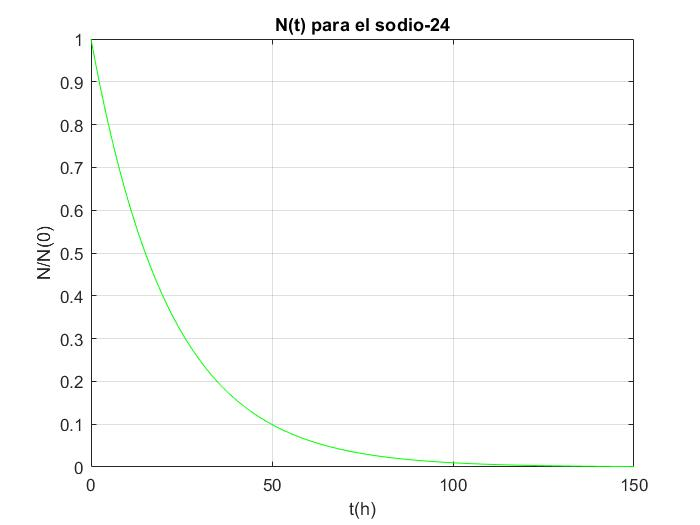
\includegraphics[scale=0.47]{imagenes/decaimiento_sodio_24.jpg}
		\caption{Gráfica del decaimiento exponencial del sodio-24 en en un intervalo de 150 horas.}
		\label{decaimientodelsodio24}
	\end{center}
\end{figure}

\begin{figure}[H]
	\begin{center}
		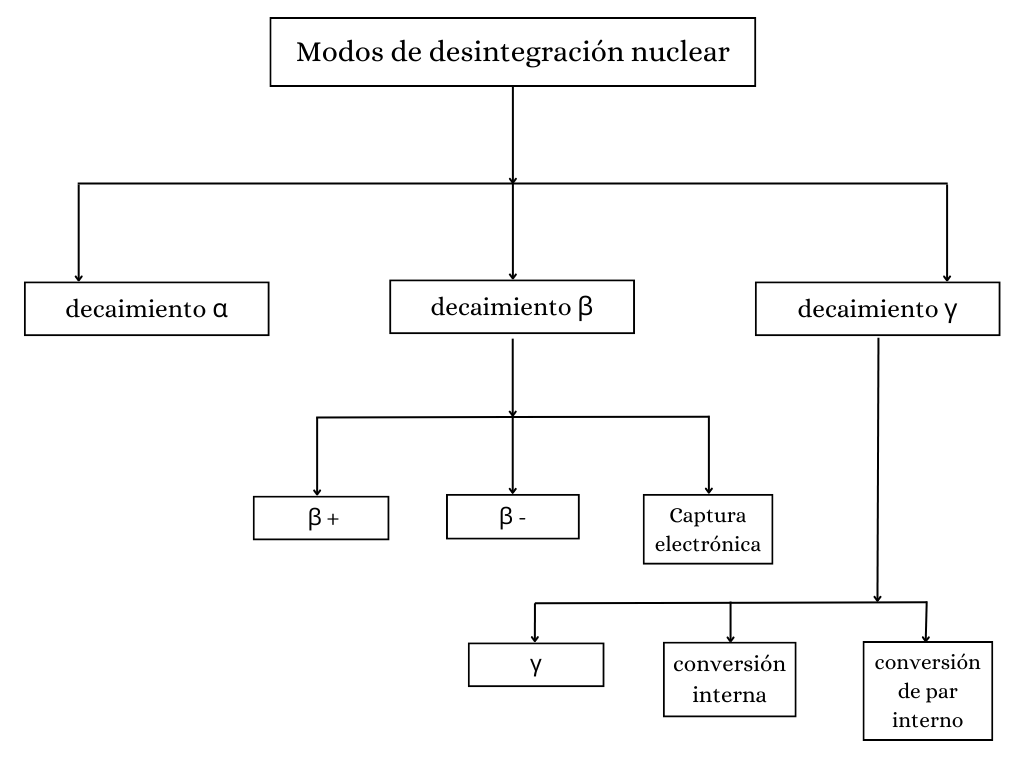
\includegraphics[scale=0.47]{imagenes/decay.png}
		\caption{Canales de desintegración para un radionúclido.}\label{channels}
	\end{center}
\end{figure}

\begin{figure}[H]
	\centering
	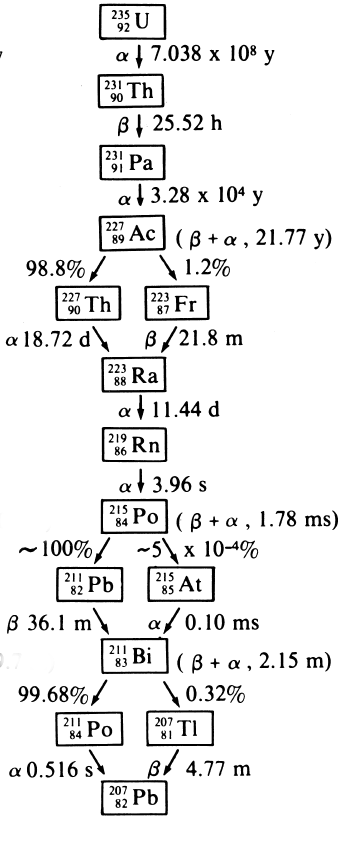
\includegraphics[scale=0.67]{imagenes/cadenaluz.png}
	\caption{Cadena de desintegración del U235 hasta Pb207. Tomada de \cite{HUBENER2003211}.}
	\label{cadenadelu235}
\end{figure}

\subsection{Gráficas de las soluciones del sistema}

\begin{figure}[H]
	\centering
	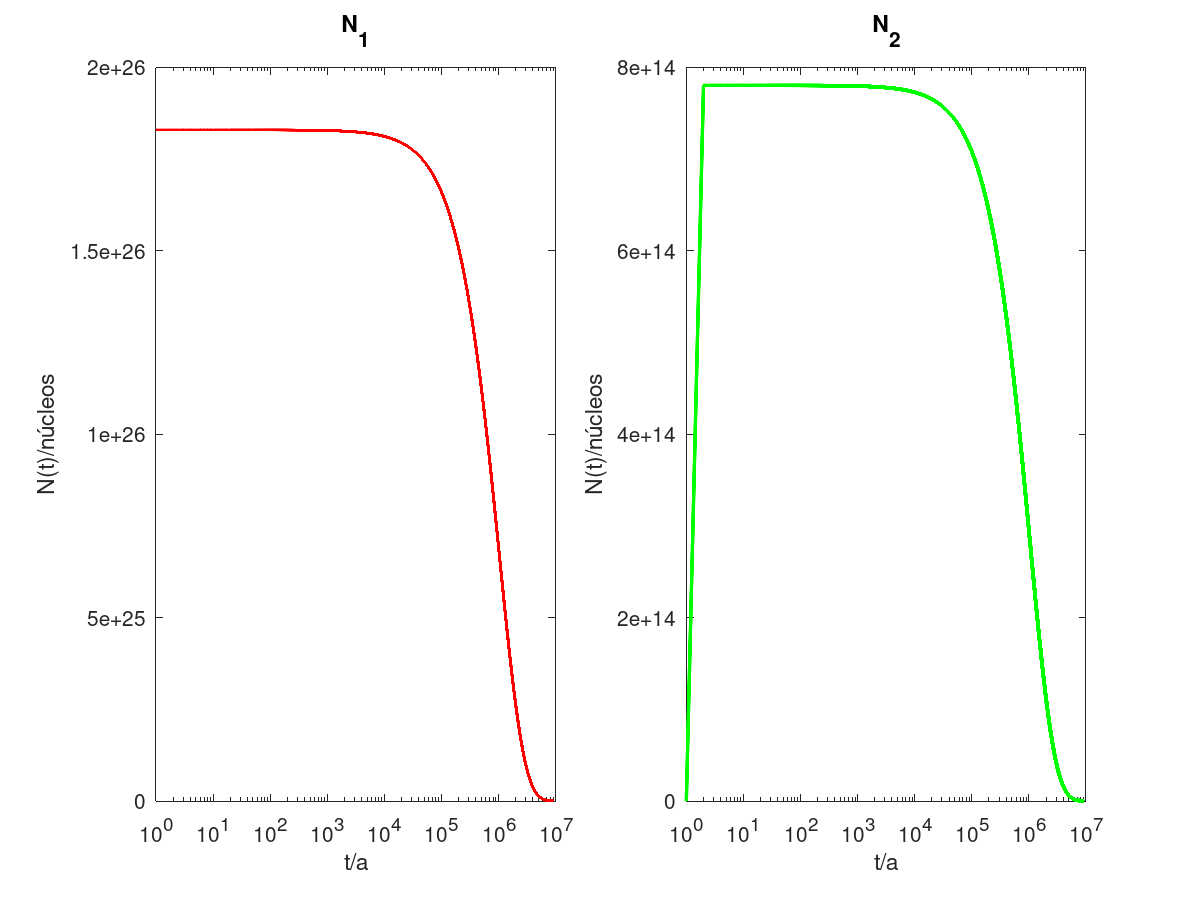
\includegraphics[scale=0.30]{/home/arias/Desktop/Research/u235_decay_chain_numsim/figuras/n1_n2.png}\label{n1n2}\caption{Curvas de desintegración de los núcleos $N_1$ y $N_2$ generadas por GNU Octave.}
\end{figure}

\begin{figure}[H]
	\centering
	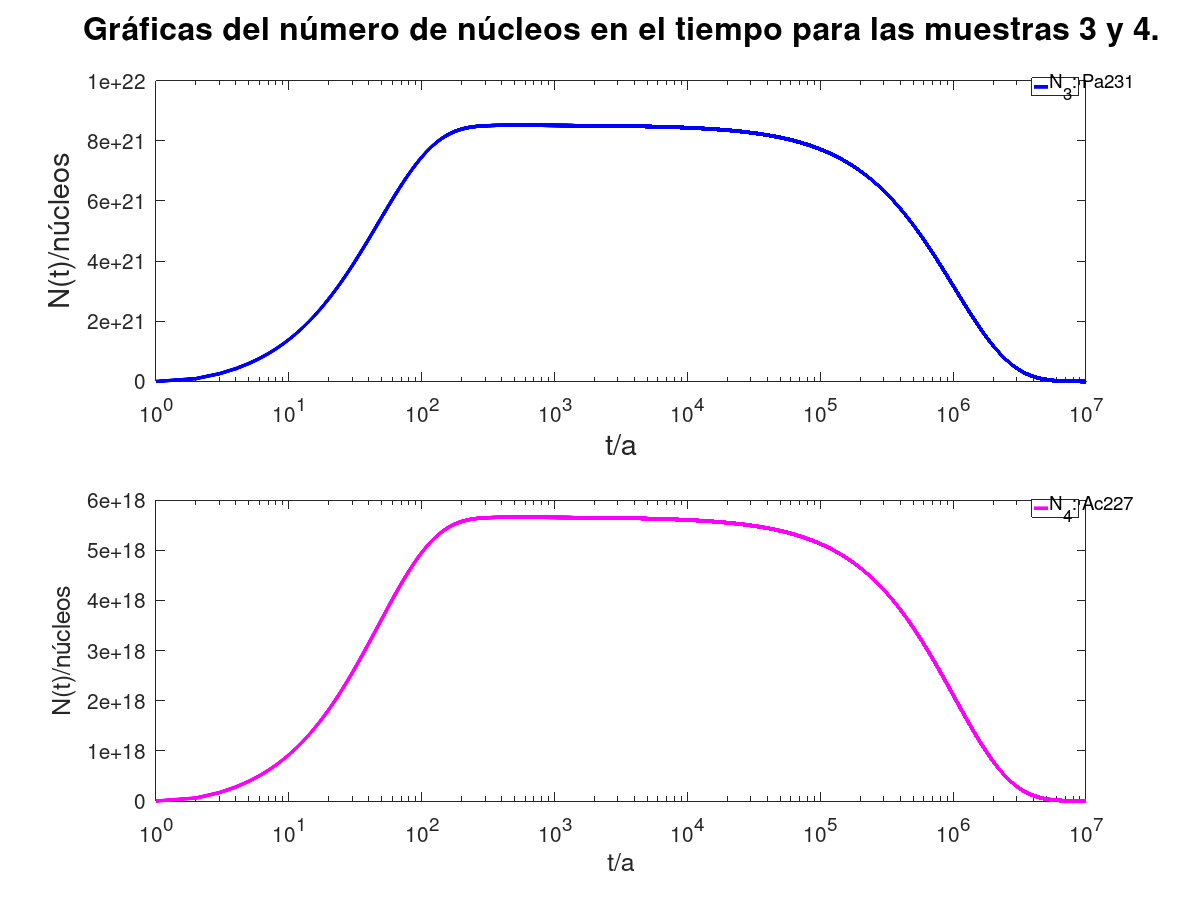
\includegraphics[scale=0.30]{/home/arias/Desktop/Research/u235_decay_chain_numsim/figuras/n3_n4.png}\label{n3n4}\caption{Curvas de desintegración de los núcleos $N_3$ y $N_4$ generadas por GNU Octave.}
\end{figure}

\begin{figure}[H]
	\centering
	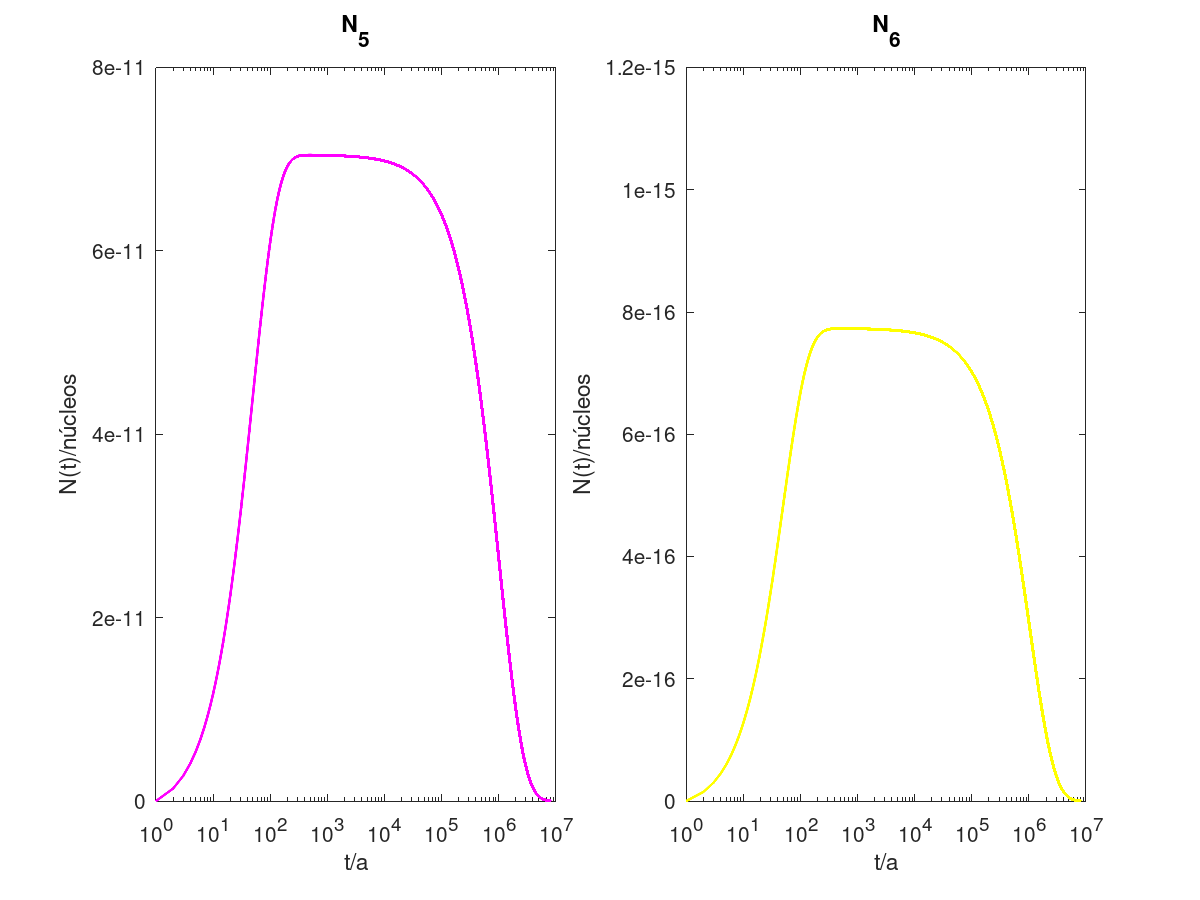
\includegraphics[scale=0.30]{/home/arias/Desktop/Research/u235_decay_chain_numsim/figuras/n5_n6.png}\label{n5n6}\caption{Curvas de desintegración de los núcleos $N_5$ y $N_6$ generadas por GNU Octave.}
\end{figure}

\begin{figure}[H]
	\centering
	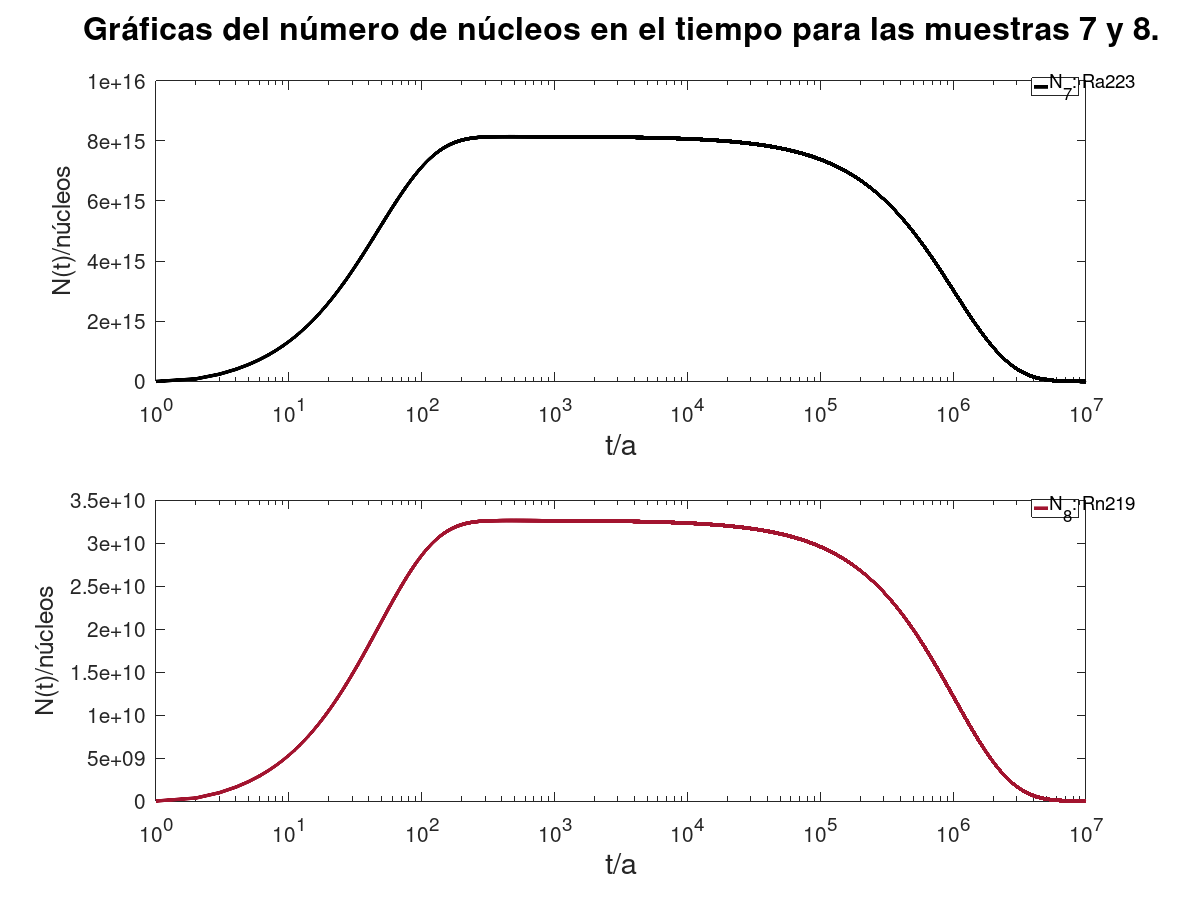
\includegraphics[scale=0.30]{/home/arias/Desktop/Research/u235_decay_chain_numsim/figuras/n7_n8.png}\label{n7n8}\caption{Curvas de desintegración de los núcleos $N_7$ y $N_8$ generadas por GNU Octave.}
\end{figure}

\begin{figure}[H]
	\centering
	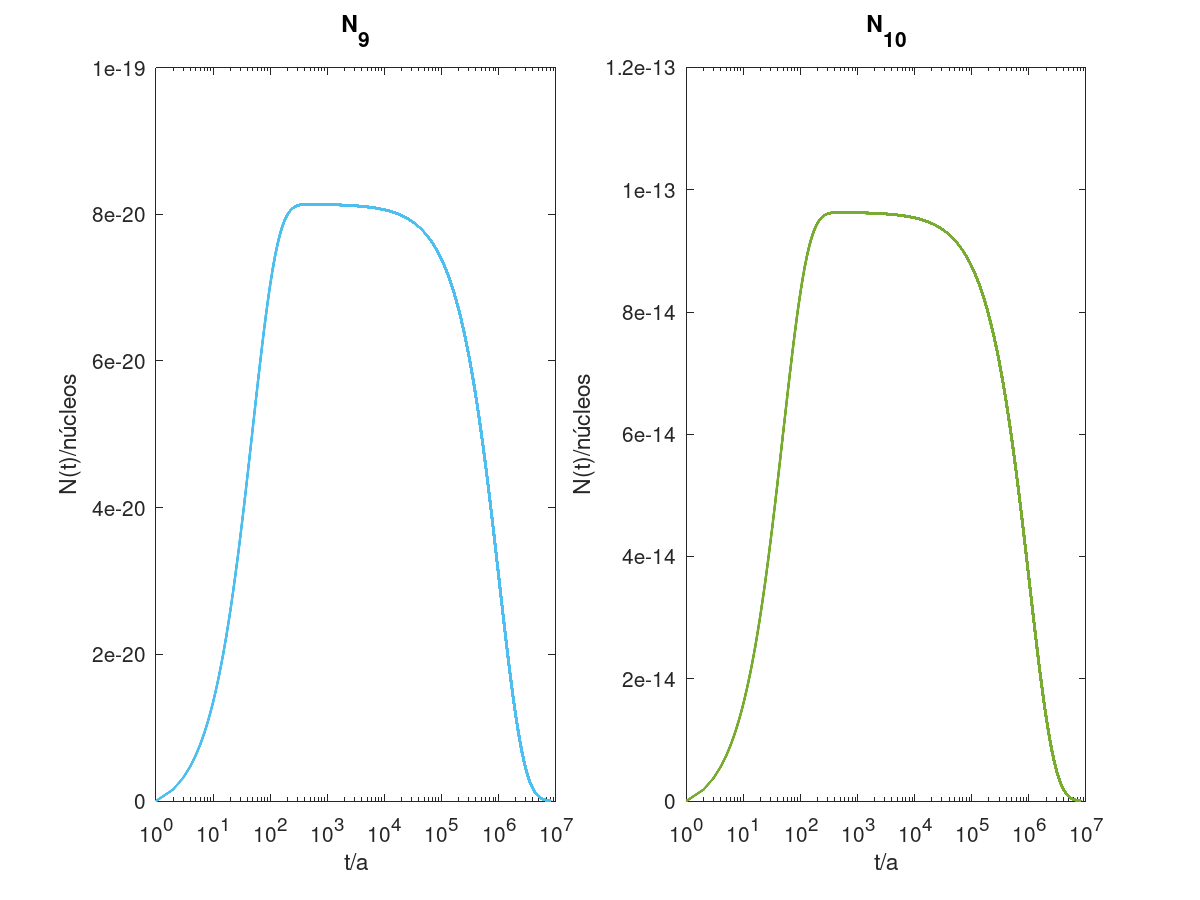
\includegraphics[scale=0.30]{/home/arias/Desktop/Research/u235_decay_chain_numsim/figuras/n9_n10.png}\label{n9n10}\caption{Curvas de desintegración de los núcleos $N_9$ y $N_{10}$ generadas por GNU Octave.}
\end{figure}

\begin{figure}[H]
	\centering
	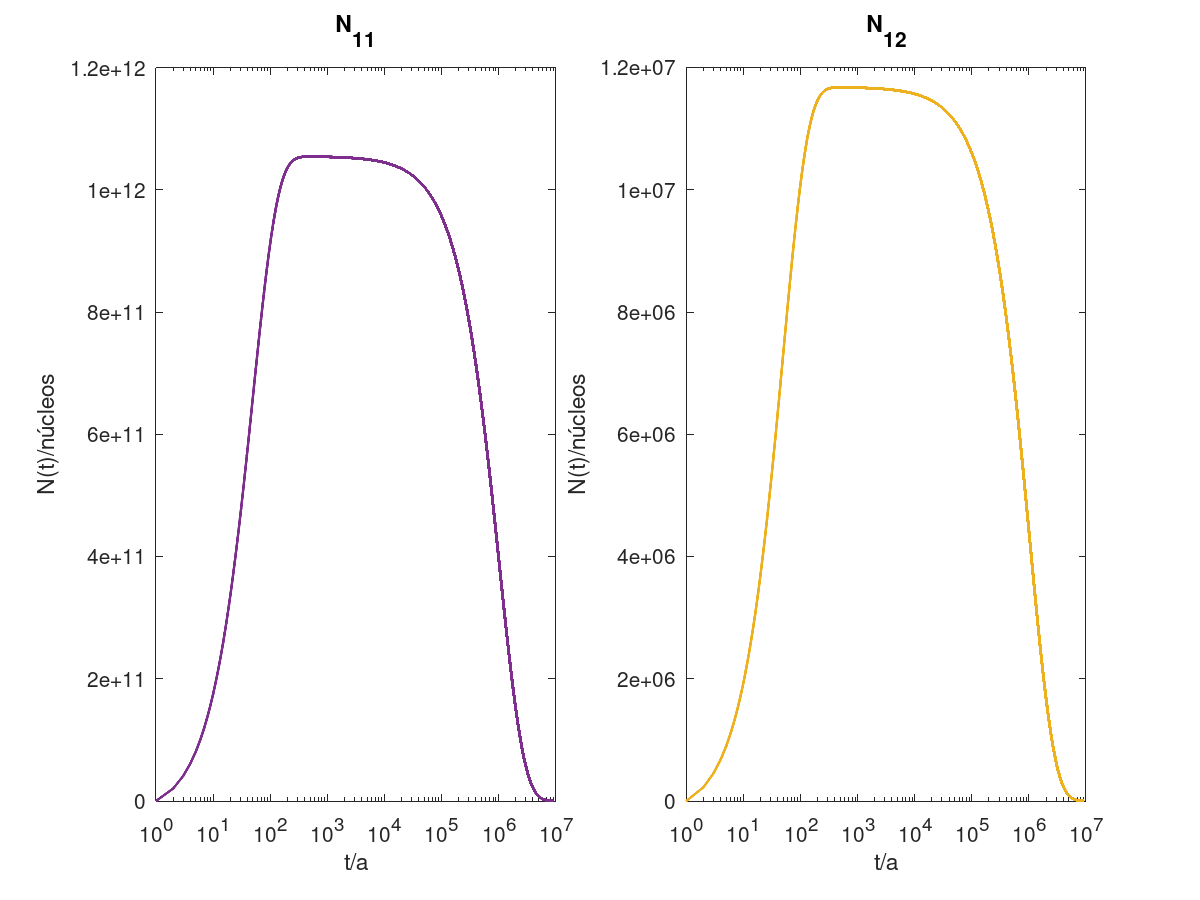
\includegraphics[scale=0.30]{/home/arias/Desktop/Research/u235_decay_chain_numsim/figuras/n11_n12.png}\label{n11n12}\caption{Curvas de desintegración de los núcleos $N_{11}$ y $N_{12}$ generadas por GNU Octave.}
\end{figure}

\begin{figure}[H]
	\centering
	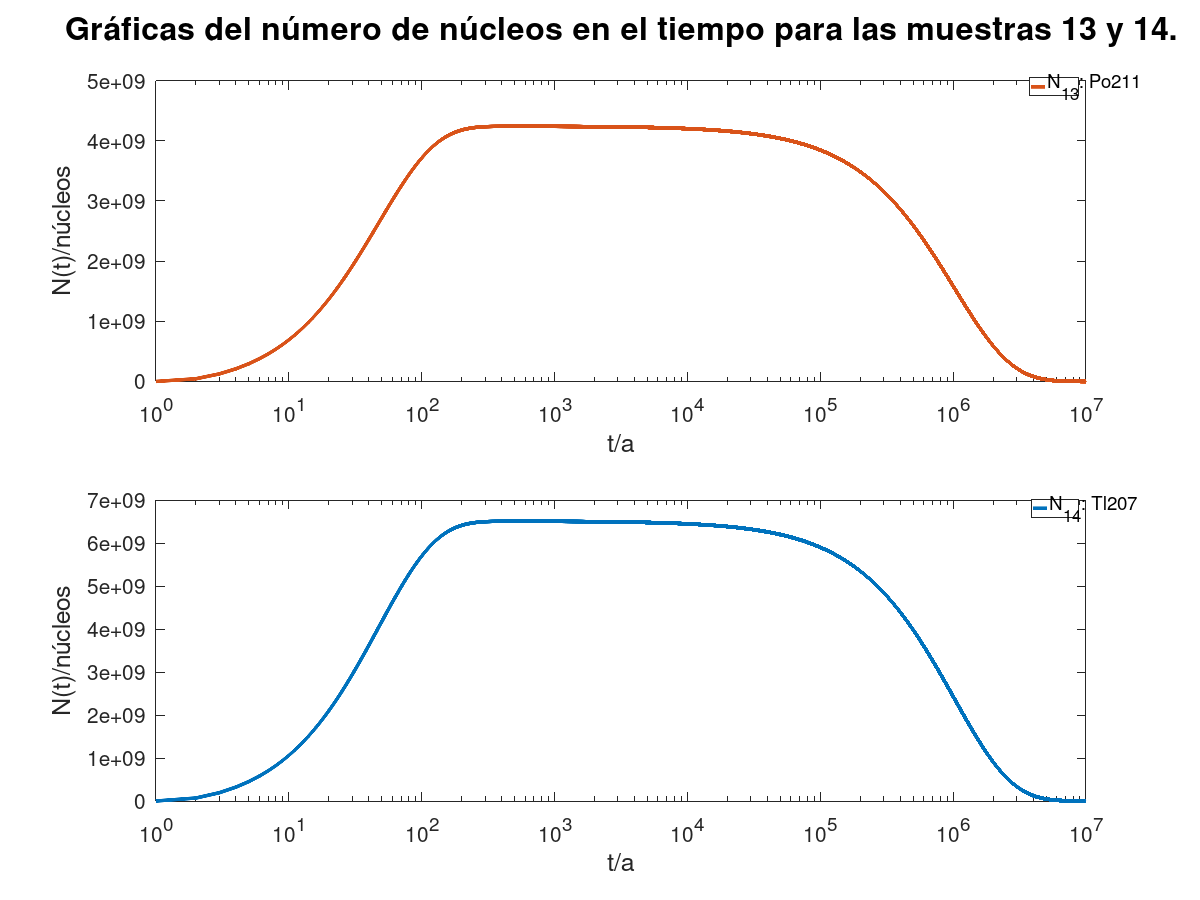
\includegraphics[scale=0.30]{/home/arias/Desktop/Research/u235_decay_chain_numsim/figuras/n13_n14.png}\label{n13n14}\caption{Curvas de desintegración de los núcleos $N_{13}$ y $N_{14}$ generadas por GNU Octave.}
\end{figure}

\begin{figure}[H]
	\centering
	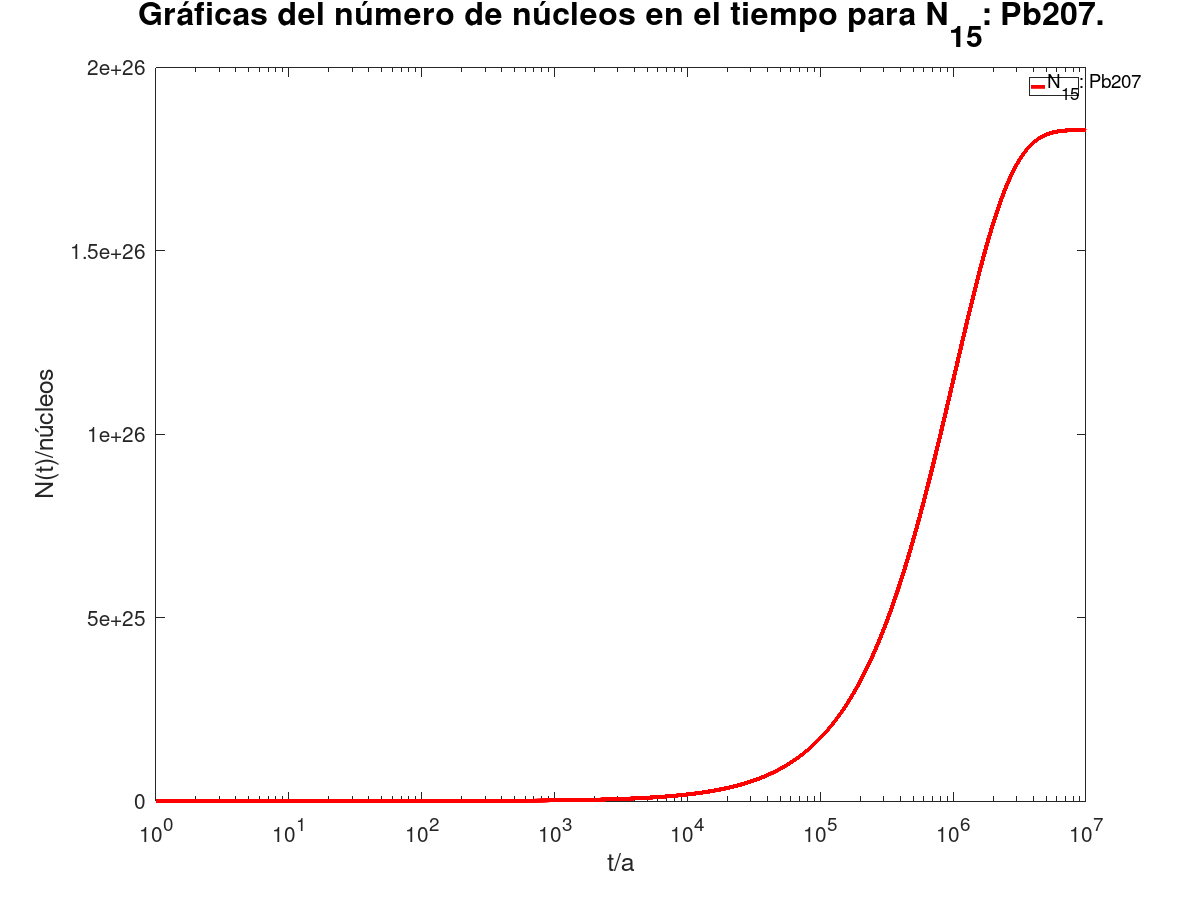
\includegraphics[scale=0.30]{/home/arias/Desktop/Research/u235_decay_chain_numsim/figuras/n15.png}\label{n15}\caption{Curva de desintegración del núcleo $N_{15}$ generada por GNU Octave.}
\end{figure}